\documentclass{llncs}
\pagestyle{plain}

\usepackage[n,advantage,operators,sets,adversary,landau,probability,notions,
logic,ff,mm,primitives,events,complexity,asymptotics,keys]{cryptocode}
\usepackage{amssymb}
\usepackage{xspace}
\usepackage[normalem]{ulem}
\PassOptionsToPackage{hyphens}{url}\usepackage{hyperref}
\usepackage{multirow}
\usepackage{footnote}
\usepackage{framed}
\usetikzlibrary{decorations.pathreplacing,calligraphy}
\makesavenoteenv{tabular}
\makesavenoteenv{table}

%% Set/unset to activate/deactivate author comments
\def\authnotes{1}

%%% Allows line-breaks in math formulae after commas
\AtBeginDocument{%
  \mathchardef\mathcomma\mathcode`\,
  \mathcode`\,="8000 
}
{\catcode`,=\active
  \gdef,{\mathcomma\discretionary{}{}{}}
}

%%%

\setcounter{tocdepth}{2}

\title{Universal Anonymous Signatures}
\author{}
\institute{}

% Custom shorthands for this paper
\definecolor{darkgreen}{rgb}{0.1,0.7,0.1}
\newcommand{\todo}[1]{{\colorbox{red}{\bf TODO:}\textcolor{red}{#1}}}
\newcommand{\doubt}[1]{{\colorbox{blue}
    {\textcolor{white}{\bf DOUBT:}}\textcolor{blue}{#1}}}
\newcommand{\response}[1]{{\colorbox{orange}{\bf RESPONSE:}
                                             \textcolor{orange}{#1}}}
\newcommand{\modified}[1]{{\textcolor{orange}{#1}}}
\newcommand{\commentwho}[2]{{\colorbox{darkgreen}{{\bf #1:}}
    \textcolor{darkgreen}{#2}}}
\newcommand{\comment}[1]{{\textcolor{orange}{\# #1}}}
%\newcommand{\note}[1]{{\colorbox{gray}{\bf NOTE:}\textcolor{gray} {#1}}}
\newcommand{\needcite}{[\colorbox{red}{?}]}
\newcommand{\figref}[1]{Fig. \ref{#1}}
\newcommand{\tabref}[1]{Table \ref{#1}}
\newcommand{\lstref}[1]{Listing \ref{#1}}
\newcommand{\secref}[1]{Section \ref{#1}}
\newcommand{\appref}[1]{Appendix \ref{#1}}
\newcommand{\defref}[1]{Definition \ref{#1}}

%\renewcommand{\qedsymbol}{$\blacksquare$}
\newcommand{\br}[1]{\ensuremath{\lbrack #1 \rbrack}}
\newcommand{\gen}[1]{\ensuremath{#1}}

\newcommand{\setind}[2]{\ensuremath{\set{#1}_{#2}}}

\mathchardef\mhyphen="2D
\def\suchthat{\ensuremath{s.t.}\xspace}

% General
\def\secpar{\ensuremath{1^\kappa}\xspace}
\def\Gen{\ensuremath{Gen}\xspace}
\def\Hash{\ensuremath{Hash}\xspace}
\def\tx{\ensuremath{tx}\xspace}
\def\getr{\ensuremath{\stackrel{\$}{\gets}}\xspace}
\def\arg{\ensuremath{arg}\xspace}
\def\msg{\ensuremath{m}\xspace}

% UC
\def\IdealF{\ensuremath{\mathcal{F}}\xspace}
\def\IdealG{\ensuremath{\mathcal{G}}\xspace}
\newcommand{\ucio}[1]{\ensuremath{\text{#1}}}
\newcommand{\uccmd}[1]{\ensuremath{\mathtt{#1}}}
\def\cmd{\ensuremath{cmd}\xspace}
\def\sid{\ensuremath{sid}\xspace}
\def\ssid{\ensuremath{ssid}\xspace}
\def\ucsend{\ucio{Send}\xspace}
\def\ucrecv{\ucio{Recv}\xspace}
\def\Sim{\ensuremath{\mathcal{S}}\xspace}
\def\Env{\ensuremath{\mathcal{E}}\xspace}
\def\Exec{\ensuremath{\text{EXEC}}}

% Signatures
\def\sig{\ensuremath{\sigma}\xspace}
\def\Sig{\ensuremath{\mathsf{S}}\xspace}
\def\IdealFSig{\ensuremath{\IdealF_{SIG}}\xspace}
\def\SIG{\ensuremath{\mathsf{SG}}\xspace}

% Hashes
\def\IdealGRO{\ensuremath{\IdealG_{RO}}\xspace}
\def\hashlist{\ensuremath{HL}\xspace}

% Key Types
\def\mpk{\ensuremath{mpk}\xspace}
\def\msk{\ensuremath{msk}\xspace}
\def\ipk{\ensuremath{ipk}\xspace}
\def\isk{\ensuremath{isk}\xspace}
\def\apk{\ensuremath{apk}\xspace}
\def\ask{\ensuremath{ask}\xspace}
\def\VK{\ensuremath{\mathsf{VK}}\xspace}

% Clock
\def\IdealGclock{\ensuremath{\IdealG_{clock}}\xspace}

% BB
\def\ldgLedger{\ensuremath{L}\xspace}
\def\IdealGledger{\ensuremath{\IdealG_{Ledger}}\xspace}
\def\IdealGdledger{\ensuremath{\IdealGledger^\delta}\xspace}
\def\ldgHonest{\ensuremath{H}\xspace}
\def\ldgMap{\ensuremath{M}\xspace}
\def\ldgState{\ensuremath{\Sigma}\xspace}
\def\ldgUtxo{\ensuremath{U}\xspace}
\def\ldgTx{\ensuremath{tx}\xspace}
\def\ldgBlock{\ensuremath{B}\xspace}
\def\ldgHead{\ensuremath{Head}\xspace}

% VDR
\def\VDR{\ensuremath{\mathsf{VDR}}\xspace}

% DIDs
\def\IdealGPKIDID{\ensuremath{\IdealG^{\P,\delta}_{\mathsf{PKIdvu}}}\xspace}
\def\did{\ensuremath{did}\xspace}
\def\DID{\ensuremath{\mathsf{DID}}\xspace}
\def\DIDCreate{\ensuremath{\DID.Create}\xspace}
\def\DIDRead{\ensuremath{\DID.Read}\xspace}
\def\DIDUpdate{\ensuremath{\DID.Update}\xspace}
\def\DIDReadLdg{\ensuremath{\mathsf{ParseLedger}}\xspace}
\def\didOp{\ensuremath{op}\xspace}
\def\didOP{\ensuremath{\mathsf{OP}}\xspace}
\def\didOWN{\ensuremath{\mathsf{OWN}}\xspace}
\def\typ{\ensuremath{t}\xspace}
\def\lbl{\ensuremath{l}\xspace}
\def\LBL{\ensuremath{L}\xspace}
\def\val{\ensuremath{v}\xspace}
\def\sval{\ensuremath{\mathbf{v}}\xspace}
\def\VAL{\ensuremath{V}\xspace}
\def\P{\ensuremath{\mathtt{P}}\xspace}
% \def\Pc{\ensuremath{\mathtt{P}_{\mathtt{C}}}\xspace}
% \def\Pu{\ensuremath{\mathtt{P}_{\mathtt{U}}}\xspace}
% \def\Pd{\ensuremath{\mathtt{P}_{\mathtt{D}}}\xspace}

% VCs
\def\VC{\ensuremath{\mathsf{VC}}\xspace}
\def\VCCreate{\ensuremath{\VC.Create}\xspace}
\def\VCPublish{\ensuremath{\VC.Publish}\xspace}
\def\VCRevoke{\ensuremath{\VC.Revoke}\xspace}
\def\VCShow{\ensuremath{\VC.Show}\xspace}
\def\VCVerify{\ensuremath{\VC.Verify}\xspace}

% Misc
\def\IdealFCA{\ensuremath{\IdealF_{CA}}\xspace}

% Atala
\def\RealPKIDIDAtala{\ensuremath{\Pi_{DID}^{Atala}}\xspace}
\def\phiDID{\ensuremath{\phi_{DID}}\xspace}
\def\MasterKey{\texttt{M}\xspace}
\def\AuthKey{\texttt{A}\xspace}
\def\CommKey{\texttt{C}\xspace}
\def\IssueKey{\texttt{I}\xspace}
\def\LMKL{\texttt{LMKL}\xspace}

%%% Local Variables: 
%%% mode: pdflatex
%%% TeX-master: "prism-protocol"
%%% End:

% Symbols for UAS
\def\UAS{\ensuremath{\mathsf{UAS}}\xspace}
\def\IGEN{\ensuremath{\mathsf{IGEN}}\xspace}
\def\OGEN{\ensuremath{\mathsf{OGEN}}\xspace}
\def\ICORR{\ensuremath{\mathsf{ICORR}}\xspace}
\def\OCORR{\ensuremath{\mathsf{OCORR}}\xspace}
\def\CCORR{\ensuremath{\mathsf{CCORR}}\xspace}
\def\HUGEN{\ensuremath{\mathsf{HUGEN}}\xspace}
\def\CUGEN{\ensuremath{\mathsf{CUGEN}}\xspace}
\def\OBTAIN{\ensuremath{\mathsf{OBTAIN}}\xspace}
\def\OBTISS{\ensuremath{\mathsf{OBTISS}}\xspace}
\def\ISSUE{\ensuremath{\mathsf{ISSUE}}\xspace}
\def\SIGN{\ensuremath{\mathsf{SIGN}}\xspace}
\def\OPEN{\ensuremath{\mathsf{OPEN}}\xspace}
\def\INSPECT{\ensuremath{\mathsf{INSPECT}}\xspace}
\def\CHALb{\ensuremath{\mathsf{SIGCHAL}_b}\xspace}
\def\OBTCHALb{\ensuremath{\mathsf{OBTCHAL}_b}\xspace}
\def\SIMSETUP{\ensuremath{\mathsf{SimSetup}}\xspace}
\def\SIMOBTAIN{\ensuremath{\mathsf{SIMOBTAIN}}\xspace}
\def\SIMSIGN{\ensuremath{\mathsf{SIMSIGN}}\xspace}
\def\SIMOPEN{\ensuremath{\mathsf{SIMOPEN}}\xspace}
\def\ATTR{\ensuremath{\mathsf{ATT}}\xspace}
\def\UATTR{\ensuremath{\mathsf{U}\ATTR}\xspace}
\def\DATTR{\ensuremath{\mathsf{D}\ATTR}\xspace}
\def\OWNR{\ensuremath{\mathsf{OWN}}\xspace}
\def\GRP{\ensuremath{\mathsf{GRP}}\xspace}
\def\ISR{\ensuremath{\mathsf{ISR}}\xspace}
\def\CCRED{\ensuremath{\mathsf{CCRD}}\xspace}
\def\IK{\ensuremath{\mathsf{IK}}\xspace}
\def\OK{\ensuremath{\mathsf{OK}}\xspace}
\def\UK{\ensuremath{\mathsf{UK}}\xspace}
\def\GK{\ensuremath{\mathsf{GK}}\xspace}
\def\PUBIK{\ensuremath{\mathsf{P}\IK}\xspace}
\def\PRVIK{\ensuremath{\mathsf{S}\IK}\xspace}
\def\PUBOK{\ensuremath{\mathsf{P}\OK}\xspace}
\def\PRVOK{\ensuremath{\mathsf{S}\OK}\xspace}
\def\PUBUK{\ensuremath{\mathsf{P}\UK}\xspace}
\def\PRVUK{\ensuremath{\mathsf{S}\UK}\xspace}
\def\II{\ensuremath{\mathsf{I}}\xspace}
\def\OO{\ensuremath{\mathsf{O}}\xspace}
\def\HI{\ensuremath{\mathsf{HI}}\xspace}
\def\CI{\ensuremath{\mathsf{CI}}\xspace}
\def\HO{\ensuremath{\mathsf{HO}}\xspace}
\def\CO{\ensuremath{\mathsf{CO}}\xspace}
\def\HU{\ensuremath{\mathsf{HU}}\xspace}
\def\CU{\ensuremath{\mathsf{CU}}\xspace}
\def\CC{\ensuremath{\mathsf{CC}}\xspace}
\def\GEN{\ensuremath{\mathsf{GEN}}\xspace}
\def\CORR{\ensuremath{\mathsf{CORR}}\xspace}
\def\SIG{\ensuremath{\mathsf{SIG}}\xspace}
\def\CSIG{\ensuremath{\mathsf{CSIG}}\xspace}
%\def\CCRED{\ensuremath{\mathsf{CC}}\xspace}
\def\secpar{\ensuremath{\kappa}\xspace}
%\def\param{\ensuremath{\param}\xspace}
\def\isk{\ensuremath{isk}\xspace}
\def\ipk{\ensuremath{ipk}\xspace}
\def\sipk{\ensuremath{\mathbf{\ipk}}\xspace}
\def\osk{\ensuremath{osk}\xspace}
\def\opk{\ensuremath{opk}\xspace}
\def\gpk{\ensuremath{gpk}\xspace}
\def\sgpk{\ensuremath{\mathbf{\gpk}}\xspace}
\def\usk{\ensuremath{usk}\xspace}
\def\upk{\ensuremath{upk}\xspace}
\def\cred{\ensuremath{crd}\xspace}
\def\scred{\ensuremath{\mathbf{\cred}}\xspace}
\def\utrans{\ensuremath{reg}\xspace}
\def\trans{\ensuremath{\mathbf{reg}}\xspace}
\def\IdentifyCred{\ensuremath{\mathsf{IdentifyCred}}\xspace}
\def\IdentifySig{\ensuremath{\mathsf{IdentifySig}}\xspace}
\def\ExtractSetup{\ensuremath{\mathsf{ExtractSetup}}\xspace}
\def\ExtractSign{\ensuremath{\mathsf{ExtractSig}}\xspace}
\def\ExtractIssue{\ensuremath{\mathsf{ExtractIssue}}\xspace}
\def\c{\ensuremath{c}\xspace}
\def\y{\ensuremath{y}\xspace}
\def\yeval{\ensuremath{y_{ev}}\xspace}
\def\tyeval{\ensuremath{\tilde{y}_{ev}}\xspace}
\def\ceval{\ensuremath{\c_{ev}}\xspace}
\def\Yeval{\ensuremath{Y_{ev}}\xspace}
\def\TYeval{\ensuremath{\tilde{Y}_{ev}}\xspace}
\def\yinsp{\ensuremath{y_{op}}\xspace}
\def\tyinsp{\ensuremath{\tilde{y}_{op}}\xspace}
\def\cinsp{\ensuremath{\c_{op}}\xspace}
\def\sig{\ensuremath{\sigma}\xspace}
\def\Sig{\ensuremath{\Sigma}\xspace}
\def\iproof{\ensuremath{\pi}\xspace}
\def\tiproof{\ensuremath{\tilde{\pi}}\xspace}
\def\Setup{\ensuremath{Setup}\xspace}
\def\IKeyGen{\ensuremath{IKG}\xspace}
\def\OKeyGen{\ensuremath{OKG}\xspace}
\def\UKeyGen{\ensuremath{UKG}\xspace}
\def\Obtain{\ensuremath{Obt}\xspace}
\def\Issue{\ensuremath{Iss}\xspace}
\def\Sign{\ensuremath{Sign}\xspace}
\def\Verify{\ensuremath{Verify}\xspace}
\def\Inspect{\ensuremath{Inspect}\xspace}
\def\Judge{\ensuremath{Judge}\xspace}
\def\ExpCorrect{\ensuremath{\Exp_{\UAS,\adv}^{corr}}\xspace}
\def\CorrectIssue{\ensuremath{CorrectIssue}\xspace}
\def\CorrectEval{\ensuremath{CorrectEval}\xspace}
\def\CorrectEvalInspect{\ensuremath{CorrectEvalInspect}\xspace}
\def\CorrectInspect{\ensuremath{CorrectInspect}\xspace}
\def\ExpExtractIssue{\ensuremath{\Exp_{\UAS,\adv}^{ext-iss}}\xspace}
\def\ExpExtractSign{\ensuremath{\Exp_{\UAS,\adv}^{ext-sig}}\xspace}
\def\ExpIdentifyCred{\ensuremath{\Exp_{\UAS,\adv}^{id-cred}}\xspace}
\def\ExpIdentifySign{\ensuremath{\Exp_{\UAS,\adv}^{id-sig}}\xspace}
\def\ExpSimAnonb{\ensuremath{\Exp_{\UAS,\adv}^{sim-anon-b}}\xspace}
\def\ExpSigAnonb{\ensuremath{\Exp_{\UAS,\adv}^{sig-anon-b}}\xspace}
\def\ExpIssAnonb{\ensuremath{\Exp_{\UAS,\adv}^{iss-anon-b}}\xspace}
\def\ExpSigAnonz{\ensuremath{\Exp_{\UAS,\adv}^{sig-anon-0}}\xspace}
\def\ExpIssAnonz{\ensuremath{\Exp_{\UAS,\adv}^{iss-anon-0}}\xspace}
\def\ExpSigAnonzo{\ensuremath{\Exp_{\UAS,\adv}^{sig-anon-01}}\xspace}
\def\ExpSigAnono{\ensuremath{\Exp_{\UAS,\adv}^{sig-anon-1}}\xspace}
\def\ExpIssAnono{\ensuremath{\Exp_{\UAS,\adv}^{iss-anon-1}}\xspace}
\def\ExpSigAnonoz{\ensuremath{\Exp_{\UAS,\adv}^{sig-anon-10}}\xspace}
\def\ExpSimAnono{\ensuremath{\Exp_{\UAS,\adv}^{sim-anon-1}}\xspace}
\def\ExpSimAnonz{\ensuremath{\Exp_{\UAS,\adv}^{sim-anon-0}}\xspace}
\def\AdvSigAnon{\ensuremath{\Adv_{\UAS,\adv}^{sig-anon}}\xspace}
\def\AdvIssAnon{\ensuremath{\Adv_{\UAS,\adv}^{iss-anon}}\xspace}
\def\AdvSimAnon{\ensuremath{\Adv_{\UAS,\adv}^{sim-anon}}\xspace}
\def\AdvIdCred{\ensuremath{\Adv_{\UAS,\adv}^{id-cred}}\xspace}
\def\AdvIdSign{\ensuremath{\Adv_{\UAS,\adv}^{id-sig}}\xspace}
\def\ExpTrace{\ensuremath{\Exp_{\UAS,\adv}^{trace}}\xspace}
\def\AdvTrace{\ensuremath{\Adv_{\UAS,\adv}^{trace}}\xspace}
\def\IssueTrace{\ensuremath{IssTrace}\xspace}
\def\IssueForge{\ensuremath{IssForge}\xspace}
\def\ExpForgeIssue{\ensuremath{\Exp_{\UAS,\adv}^{iss-forge}}\xspace}
\def\AdvForgeIssue{\ensuremath{\Adv_{\UAS,\adv}^{iss-forge}}\xspace}
\def\ExpForgeSign{\ensuremath{\Exp_{\UAS,\adv}^{sig-forge}}\xspace}
\def\AdvForgeSign{\ensuremath{\Adv_{\UAS,\adv}^{sig-forge}}\xspace}
\def\EvalForge{\ensuremath{EvForge}\xspace}
\def\EvalInspectForge{\ensuremath{EvInForge}\xspace}
\def\InspectForge{\ensuremath{InForge}\xspace}
\def\ExpNonframe{\ensuremath{\Exp_{\UAS,\adv}^{frame}}\xspace}
\def\AdvNonframe{\ensuremath{\Adv_{\UAS,\adv}^{frame}}\xspace}
\def\ExpNonframeSign{\ensuremath{\Exp_{\UAS,\adv}^{frame-sign}}\xspace}
\def\AdvNonframeSign{\ensuremath{\Adv_{\UAS,\adv}^{frame-insp}}\xspace}
\def\ExpNonframeInsp{\ensuremath{\Exp_{\UAS,\adv}^{frame-insp}}\xspace}
\def\AdvNonframeInsp{\ensuremath{\Adv_{\UAS,\adv}^{frame-insp}}\xspace}
\def\ExpExtractIssue{\ensuremath{\Exp_{\UAS,\adv}^{ext-issue}}\xspace}
\def\AdvExtractIssue{\ensuremath{\Adv_{\UAS,\adv}^{ext-issue}}\xspace}
\def\ExpExtractSign{\ensuremath{\Exp_{\UAS,\adv}^{ext-sign}}\xspace}
\def\AdvExtractSign{\ensuremath{\Adv_{\UAS,\adv}^{ext-sign}}\xspace}
\def\choose{\ensuremath{\mathsf{choose}}\xspace}
\def\guess{\ensuremath{\mathsf{guess}}\xspace}
\def\Oanonc{\ensuremath{\mathcal{O}^{anon-b}_{\choose}}\xspace}
\def\Oanong{\ensuremath{\mathcal{O}^{anon-b}_{\guess}}\xspace}
\def\OExt{\ensuremath{\mathcal{O}^{ext}}\xspace}
\def\OId{\ensuremath{\mathcal{O}^{id}}\xspace}
\def\OIssAnon{\ensuremath{\mathcal{O}^{iss-anon-b}}\xspace}
\def\OSigAnon{\ensuremath{\mathcal{O}^{sig-anon-b}}\xspace}
\def\Osimanon{\ensuremath{\mathcal{O}^{sim-anon-b}}\xspace}
\def\Otrace{\ensuremath{\mathcal{O}^{trace}}\xspace}
\def\Oforgeissue{\ensuremath{\mathcal{O}^{iss-forge}}\xspace}
\def\Oforgesign{\ensuremath{\mathcal{O}^{sig-forge}}\xspace}
\def\Oframe{\ensuremath{\mathcal{O}^{frame}}\xspace}
\def\gid{\ensuremath{\mathsf{gid}}\xspace}
\def\iid{\ensuremath{\mathsf{iid}}\xspace}
\def\oid{\ensuremath{\mathsf{oid}}\xspace}
\def\sgid{\ensuremath{\boldsymbol{\mathsf{\gid}}}\xspace}
\def\siid{\ensuremath{\boldsymbol{\mathsf{\iid}}}\xspace}
\def\uid{\ensuremath{\mathsf{uid}}\xspace}
\def\suid{\ensuremath{\boldsymbol{\mathsf{uid}}}\xspace}
\def\cuid{\ensuremath{\mathsf{uid}^*}\xspace}
\def\cid{\ensuremath{\mathsf{cid}}\xspace}
\def\scid{\ensuremath{\boldsymbol{\mathsf{cid}}}\xspace}
\def\ccid{\ensuremath{\mathsf{cid}^*}\xspace}
\def\cscid{\ensuremath{\scid^*}\xspace}
\def\csig{\ensuremath{\mathsf{\sigma}^*}\xspace}
\def\cSig{\ensuremath{\mathsf{\Sigma}^*}\xspace}
\def\LangIss{\ensuremath{\Lang_{is}}\xspace}
\def\RelIss{\ensuremath{\NIZKRel_{is}}\xspace}
\def\LangIns{\ensuremath{\Lang_{op}}\xspace}
\def\RelIns{\ensuremath{\NIZKRel_{op}}\xspace}
\def\LangVerIns{\ensuremath{\Lang_{verop}}\xspace}
\def\LangSig{\ensuremath{\Lang_{sig}}\xspace}
\def\RelSig{\ensuremath{\NIZKRel_{sig}}\xspace}
\def\fissue{\ensuremath{f_{is}}\xspace}
\def\feval{\ensuremath{f_{ev}}\xspace}
\def\rngfeval{\ensuremath{R_{ev}}\xspace}
\def\varrngfeval{\ensuremath{r_{ev}}\xspace}
\def\finsp{\ensuremath{f_{op}}\xspace}
\def\rngfinsp{\ensuremath{R_{op}}\xspace}
\def\varrngfinsp{\ensuremath{r_{op}}\xspace}
\def\famfissue{\ensuremath{\mathcal{F}_{is}}\xspace}
\def\famfeval{\ensuremath{\mathcal{F}_{ev}}\xspace}
\def\famfinsp{\ensuremath{\mathcal{F}_{op}}\xspace}
\def\Issuers{\ensuremath{\mathbb{I}}\xspace}
\def\CUASGen{\ensuremath{\Pi_{\UAS}}\xspace}
\def\trap{\ensuremath{\tau}\xspace}
\def\extract{\ensuremath{\mathsf{ex}}\xspace}
\def\extracttrap{\ensuremath{\tau_{\extract}}\xspace}
\def\sring{\ensuremath{\mathbf{ring}}\xspace}
\def\CUASRing{\ensuremath{\Pi_{\UAS}^{ring}}\xspace}
\def\CUASGS{\ensuremath{\Pi_{\UAS}^{gs}}\xspace}
\def\CUASAC{\ensuremath{\Pi_{\UAS}^{ac}}\xspace}
\def\CUASGSMDO{\ensuremath{\Pi_{\UAS}^{gsmdo}}\xspace}
\def\CUASDAC{\ensuremath{\Pi_{\UAS}^{dac}}\xspace}
\def\CUASRAC{\ensuremath{\Pi_{\UAS}^{rac}}\xspace}
\def\CUASMPS{\ensuremath{\Pi_{\UAS}^{mps}}\xspace}

%%% Local Variables: 
%%% mode: pdflatex
%%% TeX-master: "gsac.tex"
%%% End:


\begin{document}
{\def\addcontentsline#1#2#3{}\maketitle}%\maketitle
Version of \today

\section{Introduction}
\label{sec:introduction}

Identity management is one of the hardest problems in the digital domain%
\footnote{\url{https://www.maddyness.com/uk/2021/11/04/digital-identity-is-one-of-the-21st-centurys-biggest-challenges/}. Last access, August 30th, 2022.}.
It requires to address needs that are already complex on their own, such as:

\begin{itemize}
\item Establishing a connection between a digital persona and a physical one.
\item Interoperability across solutions.
\item Security and privacy, without sacrificing functionality.
\end{itemize}

As usual, the third item makes things even more complicated and, still, is
essential. Without proper handling of one's secrets, impersonation is trivial.
Without robust privacy protection mechanisms, high user adoption is unlikely,
and regulatory compliance, impossible. Yet, adding security makes systems less
usable, and adding privacy typically comes at the cost of using functionality.

From the previous, is not surprising that (privacy-preserving and secure)
digital identity has been a fertile ground for research. Indeed, at least for
the last four decades, it has been a recurring topic in the main cryptography
and security academic venues. Also, roughly during the last decade, it has
received increased attention in the industry\footnote{See, for instance, the
  Idemix and PrivacyABC projects, the W3C DID and Verifiable Credentials
  specification efforts, or the related ``anoncreds'' working group, etc.}

In fact, if one tries to get up to date with the latest advances in the domain,
a non-negligible added complexity is to navigate through the vast amount of
previous work. Quickly, seemingly incompatible systems arise, that offer a
different privacy-vs-utility tradeoff: from private systems that do not lose
utility at the cost of introducing a fully trusted third party who can revoke
anyone's privacy; to fully private systems that do not allow privacy revocation,
but lose all utility; passing through many things in between. Needing to make a
hard decission for a concrete privacy-vs-utility tradeoff is one of the big
drawbacks of existing systems.

We introduce here Universal Anonymous Signatures -- UAS, for short. UAS
is a flexible framework for privacy-preserving identities. Cryptographically,
it generalizes much work done durng the last 40 years. In UAS, identities are
sets of attested attributes, which have proven to be a powerful way to represent
physical-world identities. In addition, UAS enables that arbitrary claims are
proven based on these attributes, both at the time that a signature is verified
and, also \uline{afterwards} -- if needed and the request is granted by an
authority chosen by the signer. The claims to be proven are chosen by the
verifier (possibly jointly with the signer), but the signer is fully aware of
the information that will or may be revealed, if any. Indeed, the option to
reveal extra customizable information after the signature has been produced
enables very relevant use cases and, as we will see, makes a big difference in
addressing the privacy-vs-utility tradeoff. Finally, UAS is compatible with
industry efforts that focus on interoperability, such as W3C's Verifiable
Credentials or Anoncreds.

%%% Local Variables:
%%% mode: latex
%%% TeX-master: "uas-onepager"
%%% End:

\section{How Does It Work?}
\label{sec:functionality}

In UAS, there are three types of entities: issuers, users, and openers. However,
cryptographically speaking, users and issuers are the same, with the only
exception that issuers advertise their public keys, and policy for issuance.

Users receive credentials from issuers -- a user can own multiple credentials,
even from the same issuer. Then, users leverage (one or more of) these
credentials to produce a signature. As part of producing a signature, users
may need to reveal arbitrary facts related to their credentials and, in
addition, specify an opener. If the need arises, this opener can extract further
information from the signature and involved credentials, in a process that is
known as \emph{opening} a signature. Crucially, no more information than what
the user chooses to reveal can be learned from the signature; yet, the verifier
gets full certainty that the signature comes from a user with a (set of) valid
credential(s). This high-level usage is defined in \figref{fig:functionality}

\begin{figure}[ht!]
  \centering
  % \input{figures/functionality-op.tex}
  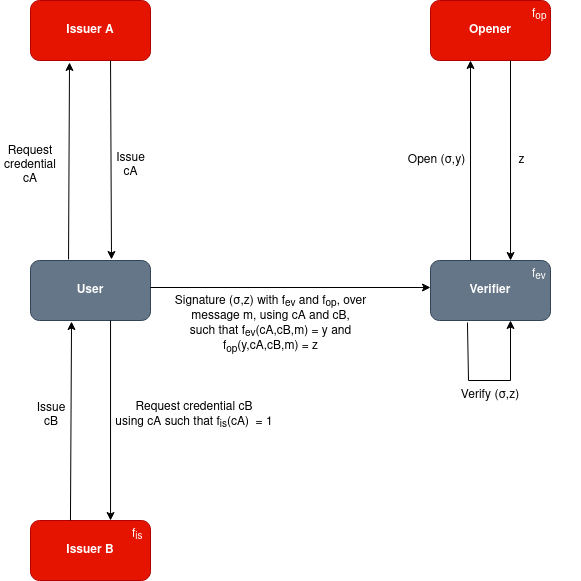
\includegraphics[width=0.8\textwidth]{figures/uas-functionality.png}
  \caption{Sketch of the functionality in UAS schemes, and how the main actors
    interact through this functionality.}
  \label{fig:functionality}
\end{figure}

What makes UAS flexible, though, is the possibility to configure even on a
per-signature basis, the information that will be revelealed, at what time. We
do this via three \emph{functional placeholders}:

\begin{description}
\item[Issuance functions, \fissue:] Issuers are required to specify what
  conditions need to be satisfied by users asking them for credentials. This is
  especially useful when a user wants (or needs) to leverage previously obtained
  credentials (from the same or a different issuer) in order to support its new
  request.
\item[Signature evaluation functions, \feval:] To produce a signature, verifiers
  require that signers prove arbitrary facts over (a subset of) their
  credentials, including revealing specific attributes. This requirement is
  specified, on a per-signature basis, via a signature evaluation function,
  which may also be dependent on the signed message.
\item[Opening functions, \finsp:] On certain scenarios, after a signature is
  produced by its signer, additional information may be required. Opening
  functions control what information can be extracted in such cases, dependent
  on the signer's credentials, the signed message and, also, on the output of
  the evaluation function. In any case, only openers chosen by the signer will
  be able to extract this information.
\end{description}

In a nutshell, UAS provides the general framework for theoretical security and
privacy analysis -- and the $(\fissue,\feval,\finsp)$ functions define the
actual utility-vs-privacy tradeoff that is achieved. Importantly, since these
functions depend on user-private data, they have to be computed by the user.
But, at the same time, issuers, verifiers, and openers need to have certainty
that they have been computed correctly. Thus, zero-knowledge proofs%
\footnote{See, for instance, the Wikipedia entry, for a gentle introduction to
  the topic: \url{https://en.wikipedia.org/wiki/Zero-knowledge_proof}. Last
  access, August 30th, 2022.} play a crucial role in UAS.

%%% Local Variables:
%%% mode: latex
%%% TeX-master: "uas-onepager"
%%% End:

\input{use-cases.tex}
\section{Where Are We?}
\label{sec:status}

Currently, we are completing our first iteration of foundational research. We
have a formal security model, generic construction, and security proofs for our
construction. All of them are being peer-reviewed.
This means that we have a solid common ground from which we can
start building concrete instantiations of UAS (such as those in
\secref{sec:use-cases}), and evaluate their performance in the real world.

Moreover, we are also beginning to work on integrating UAS within Atala Prism%
\footnote{\url{https://atalaprism.io}. Last access, August 30th, 2022.}, the
Self-Sovereign Identity (SSI) product from IOG\footnote{\url{https://iog.io}.
  Last access, August 30th, 2022.}, built atop of Cardano%
\footnote{\url{https://cardano.org}. Last access, August 30th, 2022.}, and
compliant with the most relevant specifications in the SSI domain.

%%% Local Variables:
%%% mode: latex
%%% TeX-master: "uas-onepager"
%%% End:


\bibliographystyle{splncs04}
\bibliography{uas-onepager}

\end{document}

%%% Local Variables:
%%% mode: latex
%%% TeX-master: "uas-onepager"
%%% End:
